\documentclass{beamer}
%% Possible paper sizes: a0, a0b, a1, a2, a3, a4.
%% Possible orientations: portrait, landscape
%% Font sizes can be changed using the scale option.
\usepackage[size=a0,orientation=portrait,scale=1.8]{beamerposter}
\usetheme{LLT-poster}
% \usecolortheme{ComingClean}
\usecolortheme{Entrepreneur}
% \usecolortheme{ConspiciousCreep}  %% VERY garish.

\usepackage[utf8]{inputenc}
\usepackage[T1]{fontenc}
\usepackage{libertine}
\usepackage[scaled=0.92]{inconsolata}
\usepackage[libertine]{newtxmath}

\usepackage{mwe}
\usepackage{subfig}
\usepackage{pifont} % pro pekne znacky http://ctan.org/pkg/pifont
\newcommand{\cmark}{\ding{51}} % pekne znacky
\newcommand{\xmark}{\ding{55}} % pekne zncky§

% \usebackgroundtemplate{\tikz\node[opacity=0.1]{\includegraphics[width=\paperwidth,height=\paperheight]{./Pics/world.png}};}

% \title{\raisebox{\heightof{B)}-\height+7mm}{\includegraphics[height=1.3em]{img/beacon-network-short.png}}\#filterbubble}
\title{\#filterbubble}
\author[dostal.jakub@outlook.com]{F. Sandroni, J. Dostal}
% Optional foot image
% \footimage{\includegraphics[width=2.1em]{img/ga4gh.png}}


\begin{document}
\begin{frame}[fragile]
\begin{columns}[T]
% #############################################################################
% #############################################################################
% #############################################################################
% First Column
\begin{column}{.33\textwidth}

\begin{block}{Filter Bubble}
    \center
    \begin{large}\textbf{Living in one's own information environment.}\end{large}
    \vspace{0.8cm}
    \begin{itemize}
        \item occures on social networks
        \item caused by preferential algorithms
        \item first mentioned by Eli Pariser (2011)
    \end{itemize}
\end{block}
% #############################################################################
\begin{blankblock}{1. Twitter}
	\begin{itemize}
		\item microblogging platform
        \item \textbf{following, followers} system
		\item Twitter API is suitable data source
	\end{itemize}
	\center
	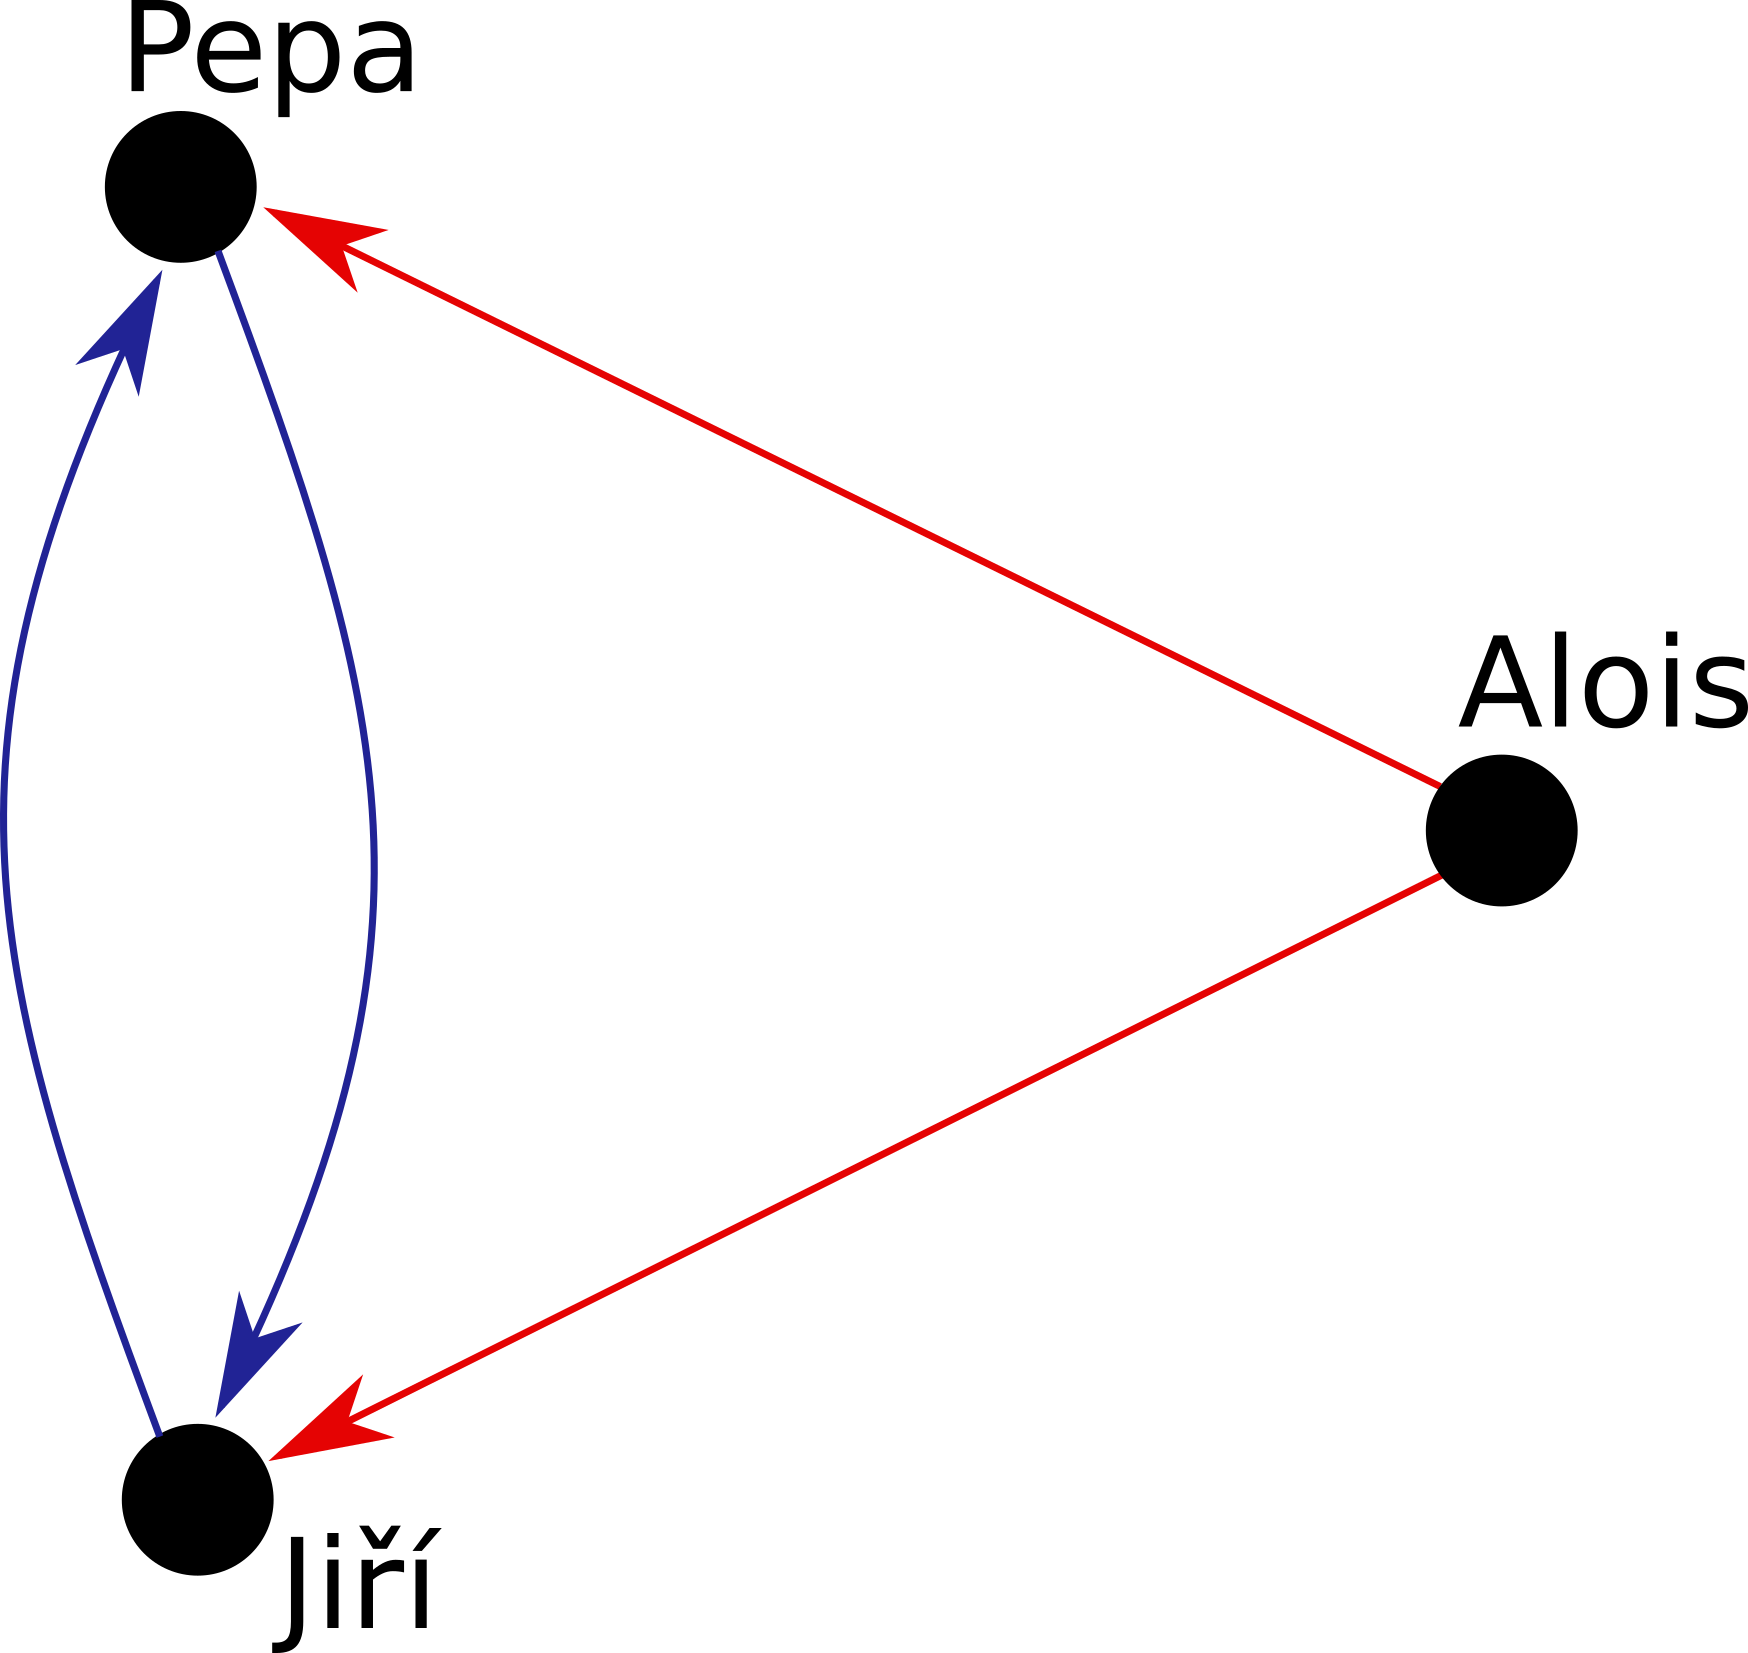
\includegraphics[scale=0.55]{./Pics/pepa.png}
\end{blankblock}
% #############################################################################
\begin{blankblock}{2. Studied groups selection}
    \begin{columns}
        \begin{column}{.6\textwidth}
            \begin{itemize}
                \item random sample from followers of the significant group
            \end{itemize}
        \end{column}
        \begin{column}{.4\textwidth}
            \center
            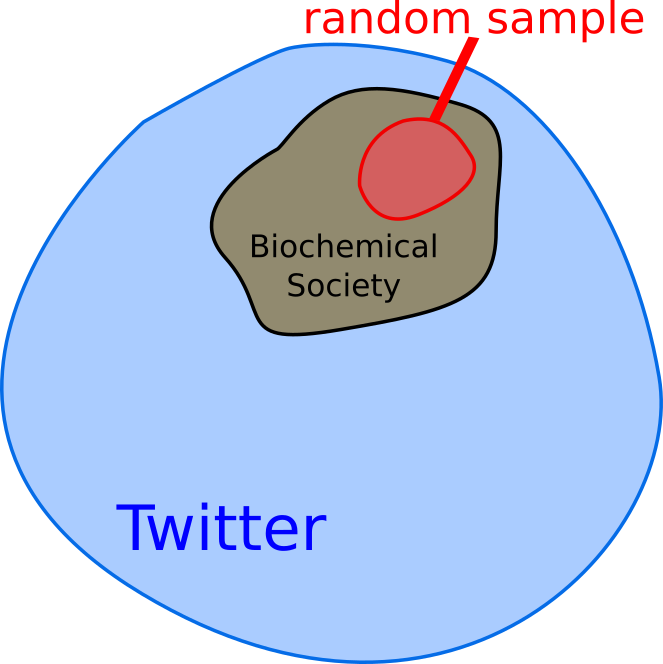
\includegraphics[scale=0.45]{./Pics/sets.png}
        \end{column}
    \end{columns}
    \center
    $\text{Twitter} \rightarrow \text{Biochemical Society} \rightarrow \text{\textbf{studied people}}$
\end{blankblock}
% #############################################################################
\begin{blankblock}{3. Tweets collection}
    \begin{columns}
    \column{.5\textwidth}
    	\begin{itemize}
            \item analysing content affecting the studied people
    	\end{itemize}
    \column{.5\textwidth}
    	\center
    	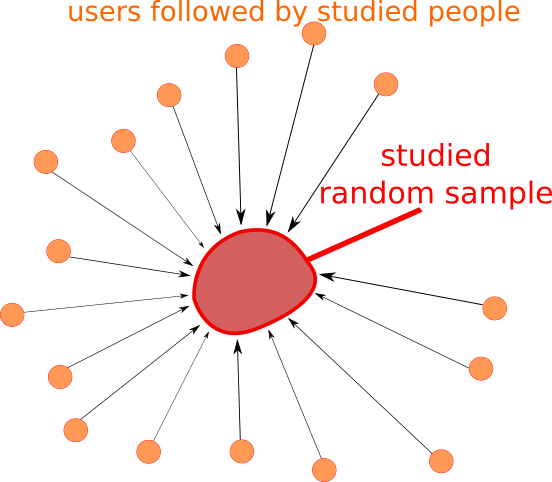
\includegraphics[scale=0.65]{./Pics/followers.png}
    \end{columns}
    \vspace{0.8cm}
    \begin{itemize}
        \item i. e. content from \textbf{followed people}
    \end{itemize}
\end{blankblock}
% #############################################################################
\begin{blankblock}{4. Tweets filtering}
\begin{itemize}
    \item filter only tweets on given topic
\end{itemize}
\vspace{0.3cm}
Keyword \textbf{"Trump"}:
\vspace{1cm}
\begin{itemize}\centering
    \item[\textcolor{black}{\xmark}] I had fish and chips for lunch.
    \item[\textcolor{black}{\cmark}] I'm glad Donald \textbf{Trump} is the president of the USA.
    % \item[\textcolor{black}{\xmark}] The president of the USA is a gentleman.
\end{itemize}
\end{blankblock}
% #############################################################################
\begin{blankblock}{5. Sentimental analysis}
\begin{itemize}
    \item measure sentiment of collected tweets
    \item \textbf{positive} vs. \textbf{negative} tweets
\end{itemize}
\center
\textit{Donald Trump is a terrible person.}\\
\textbf{(0.14)}\\
\vspace{0.5cm}
\textit{Donald Trump is a great person.}\\
\textbf{(0.95)}
\end{blankblock}

\end{column}
% #############################################################################
% #############################################################################
% #############################################################################
% Second Column
\begin{column}{.63\textwidth}
% #############################################################################
\begin{customalertblock}{Motivation}
    \begin{columns}
        \begin{column}{.5\textwidth}
            \begin{large}\textbf{Threats for democracy:}\end{large}
            \vspace{0.5cm}
            % \center
            % content \textbf{homogeneity}\\
            % $\Downarrow$\\
            % loss of objectivity\\
            % $\Downarrow$\\
            % \textbf{radicalization}
            \begin{enumerate}
                \item content \textbf{homogeneity}
                \item loss of objectivity
                \item \textbf{radicalization}
            \end{enumerate}
        \end{column}
        \begin{column}{.5\textwidth}
            \begin{large}\textbf{Goals:}\end{large}
            \vspace{0.5cm}
            \begin{itemize}
                \item filter bubble detection
                \item filter bubble quantification
            \end{itemize}
        \end{column}
    \end{columns}
    \vspace{1cm}
    Content homogeneity is a huge \textbf{threat for democratic systems}. Our aim is to develop a new method for \textbf{detecting and measuring} \textit{Filter Bubble} effects. This would provide us a new way to \textbf{study and defend from negatives} of \textit{Filter Bubble}.
\end{customalertblock}
% #############################################################################
\begin{block}{Measurements}
    \begin{columns}
        \column{0.5\textwidth}
            \underline{\textbf{Studied groups:}}
            \vspace{1cm}
            \begin{itemize}
                \item Hillary Clinton's supporters
                \item Donald Trump's supporters
            \end{itemize}
        \column{0.5\textwidth}
            \underline{\textbf{Topics:}}
            \vspace{1cm}
            \begin{itemize}
                \item Hillary Clinton
                \item Donald Trump
            \end{itemize}
    \end{columns}
    % \vspace{-2.3cm}
    \begin{columns}
        \column{0.5\textwidth}
            \begin{figure}
                \centering
                \captionsetup{justification=centering,margin=2cm}
                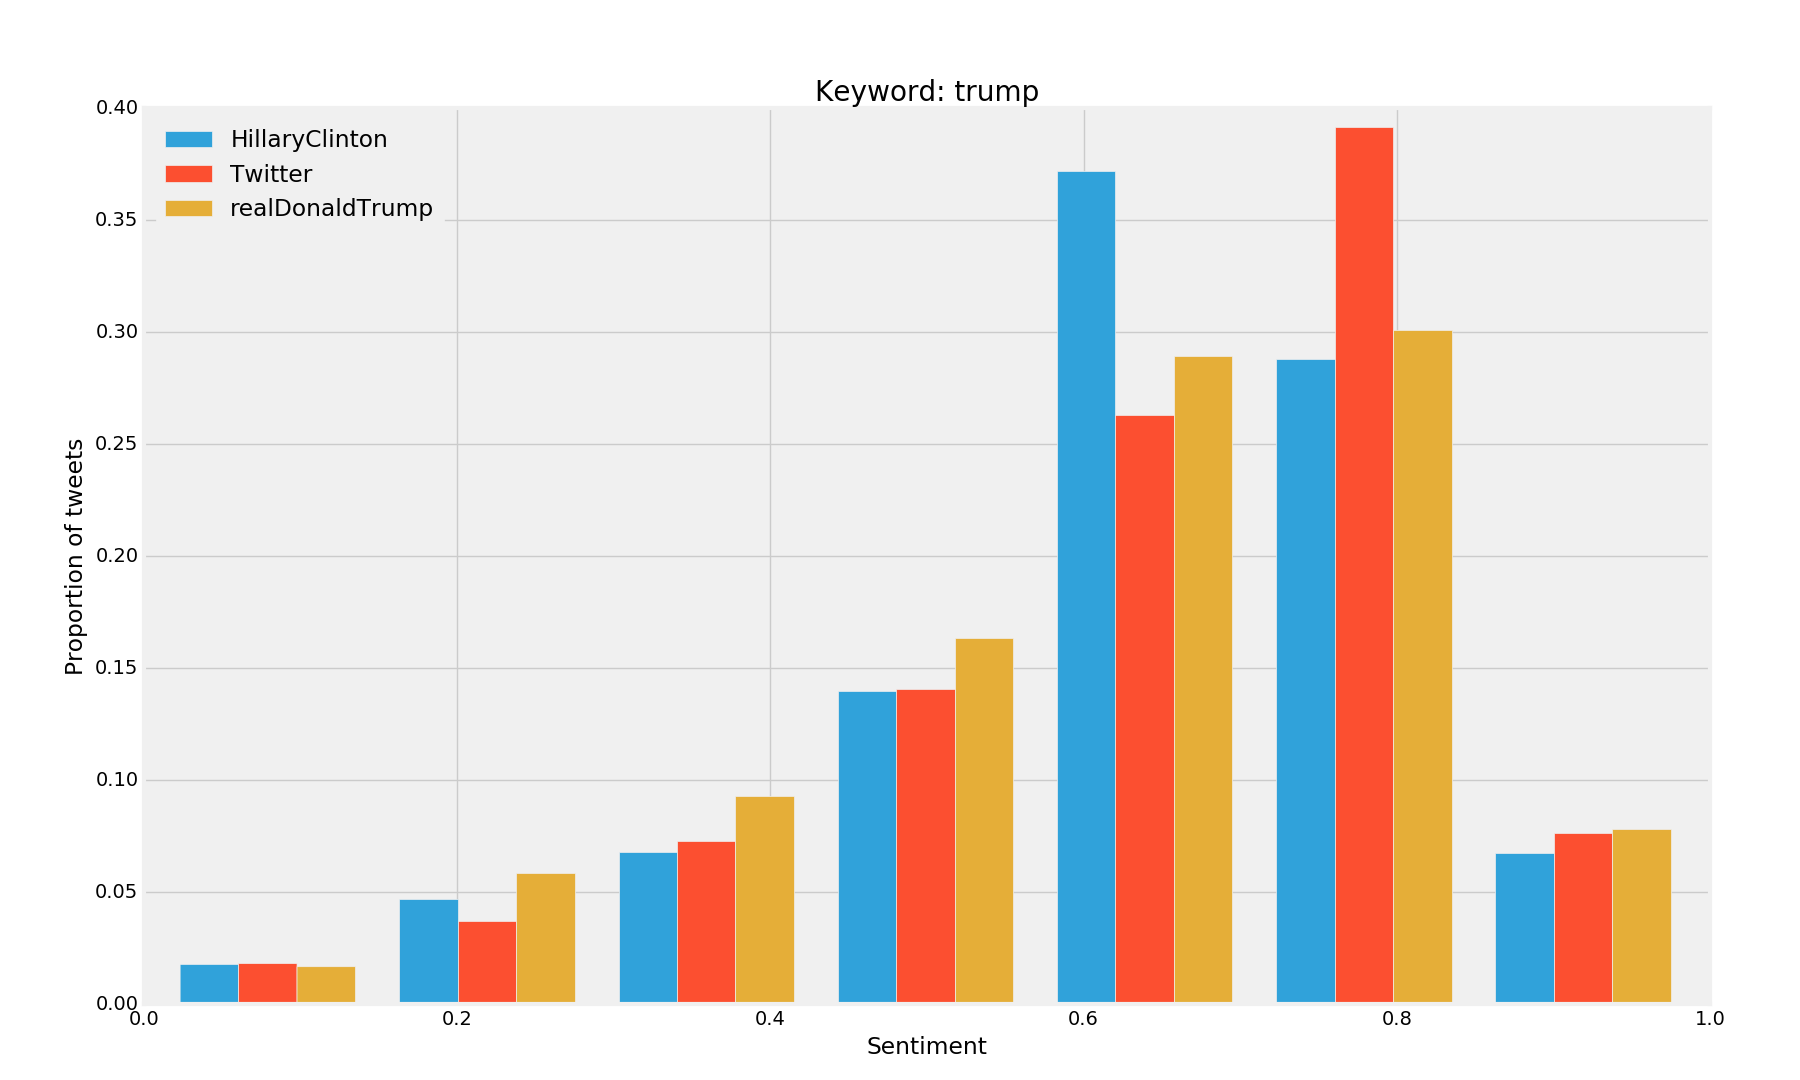
\includegraphics[scale=0.5]{./Pics/hist-trump.png}
                \caption*{Normalized sentiment histogram for topic \textit{Donald Trump}.}
            \end{figure}
        \column{0.5\textwidth}
            \begin{figure}
                \centering
                \captionsetup{justification=centering,margin=2cm}
                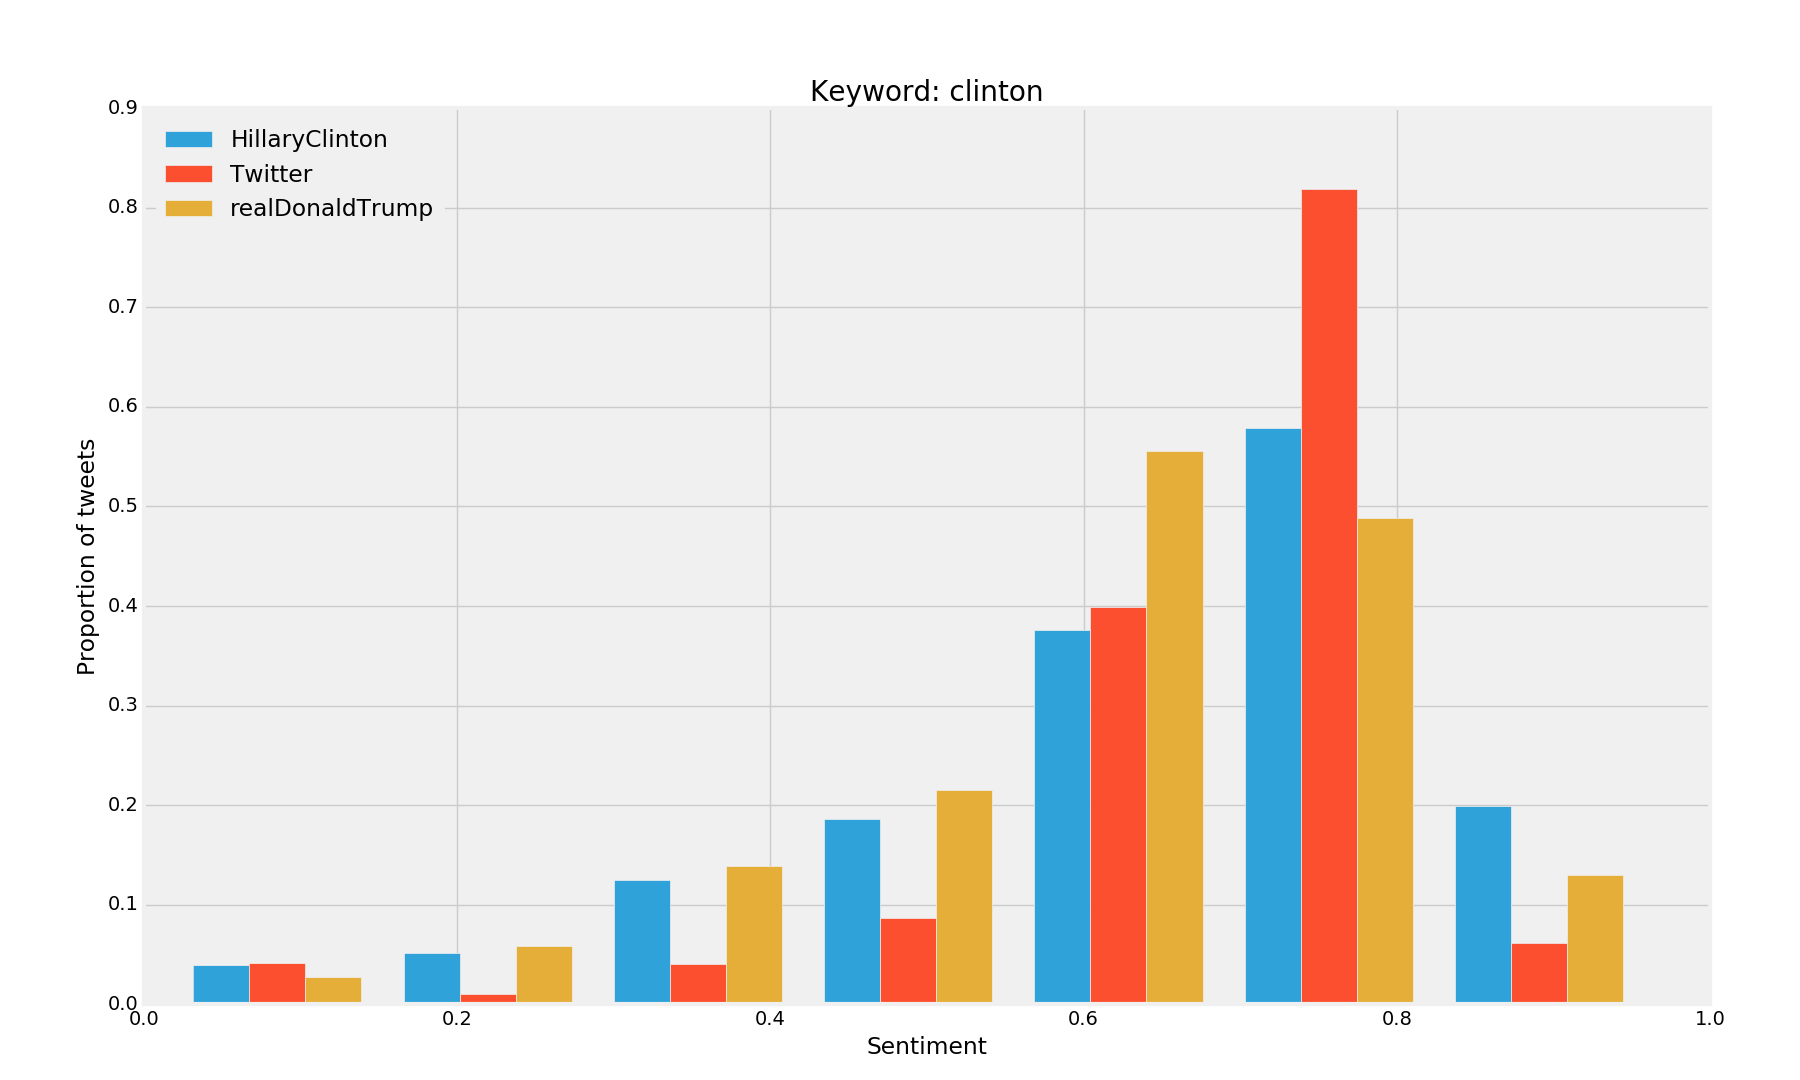
\includegraphics[scale=0.5]{./Pics/hist-clinton.png}
                \caption*{Normalized sentiment histogram for topic \textit{Hilary Clinton}.}
            \end{figure}
    \end{columns}
\end{block}
% #############################################################################
\begin{block}{Proposed measure}
    We define group affected by \textit{Filter Bubble} as a group that lays in different information environment than randomly sampled group.
    \vspace{-2cm}
    \begin{columns}
        \column{0.5\textwidth}
            \begin{figure}
                \centering
                \captionsetup{justification=centering,margin=1cm}
                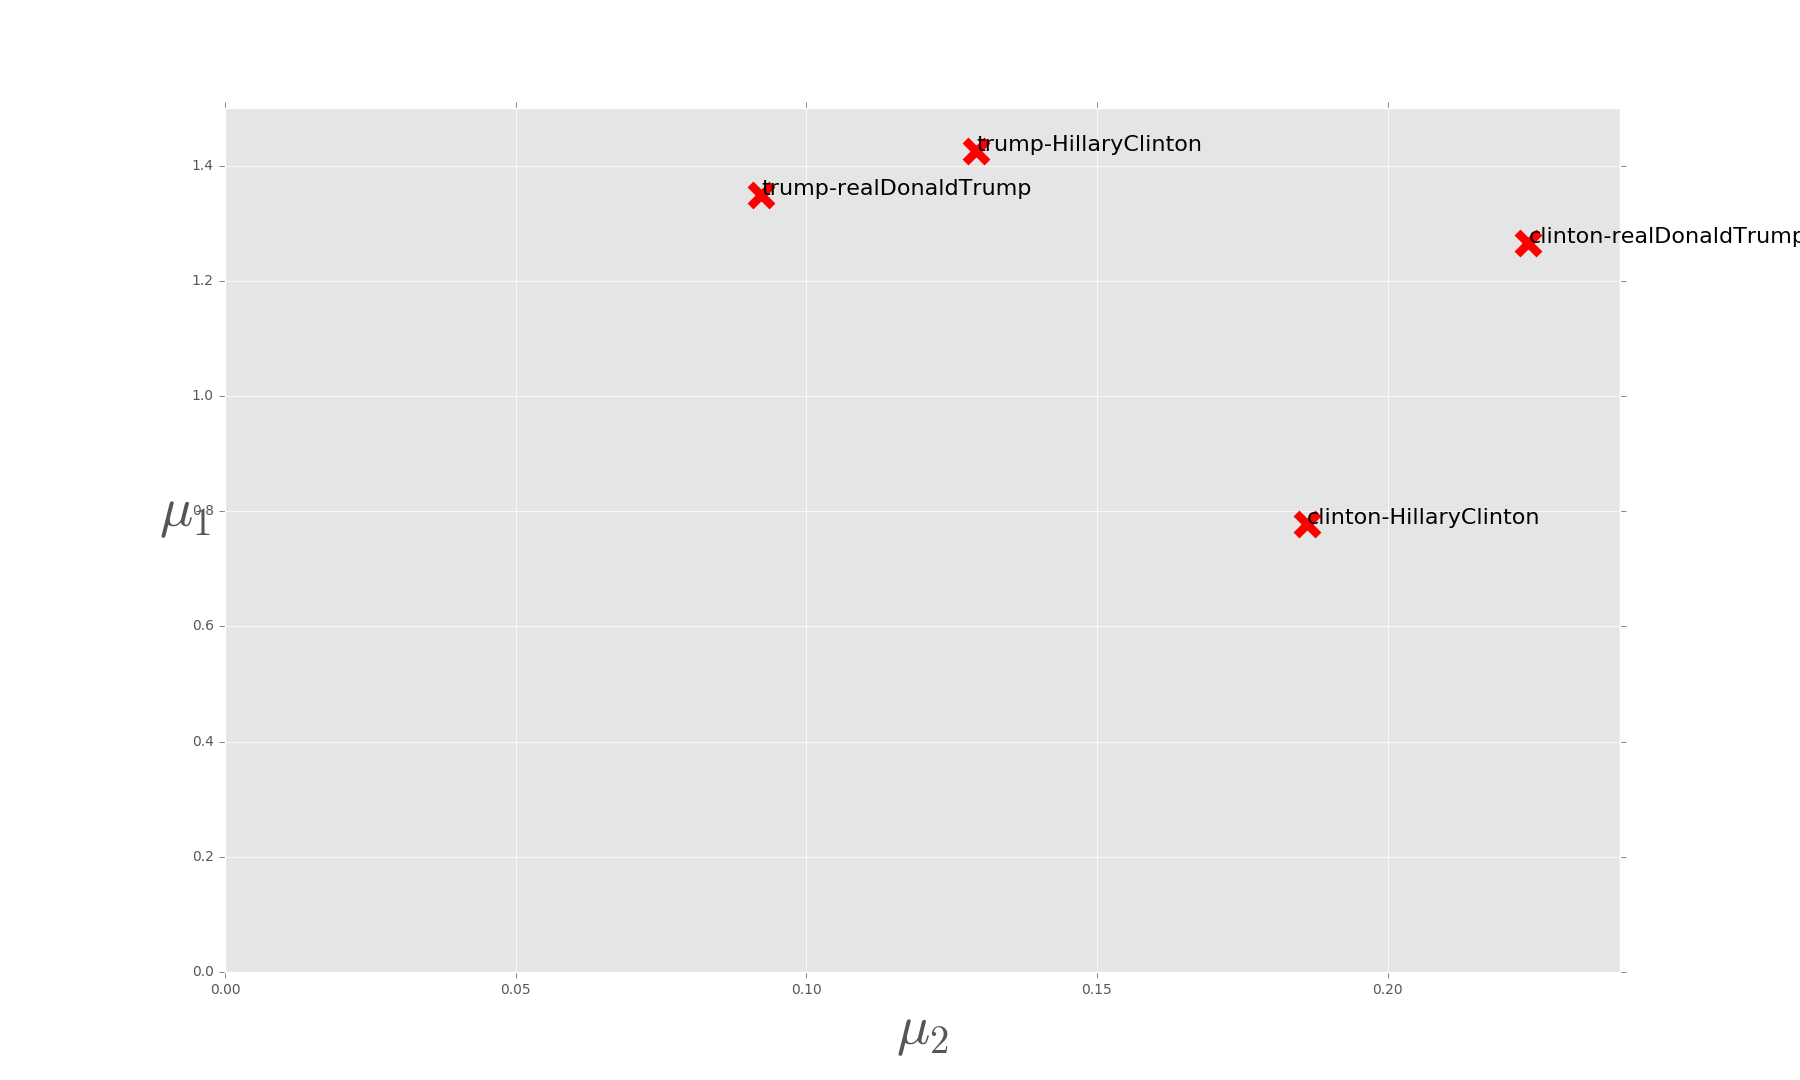
\includegraphics[scale=0.585]{./Pics/metric-L2-1Q.png}
                \caption*{Phase diagram of our measurements.}
            \end{figure}
        \column{0.5\textwidth}
            The environment may differ from average in two major ways:
            \vspace{1cm}
            \begin{enumerate}
                \item the \textbf{number of tweets} on given topic ($\mu_1$),
                \item \textbf{sentiment distribution} ($\mu_2$).
            \end{enumerate}
            \vspace{1cm}
            \textbf{Further from origin} means they receive \textbf{less balanced} information.
    \end{columns}
    \begin{columns}
        \column{0.5\textwidth}
            \begin{itemize}
                \item $\mu_1$: distance of proportion of tweets on given topic from random sample
                \item $\mu_1(G) = \frac{|p_T - p_G|}{p_t}$
            \end{itemize}
        \column{0.5\textwidth}
            \begin{itemize}
                \item $\mu_2$: distance of sentiment histogram of group $G$ from random sample ($T$)
                \item $\mu_2(G) = \sqrt{\sum_{i}{\left(S_T^i - S_G^i\right)^2}}$
            \end{itemize}
    \end{columns}
\end{block}
% #############################################################################
\begin{customalertblock}{Conclusion}
    \underline{\textbf{We have achieved:}}
    \vspace{1cm}
    \begin{enumerate}
        \item To the best of our knowledge - \textbf{the first measure} of \textit{Filter Bubble} proposed.
        \item Large scale measurements $\rightarrow$ data \textbf{noise reduction}.
        \item More \textbf{straightforward} than traditional research.
    \end{enumerate}
    \vspace{0.5cm}
    \underline{\textbf{Future plans:}}
    \vspace{1cm}
    \begin{enumerate}
        \item \textbf{Real world} usage.
        \item Modify methodology for use \textbf{outside the Twitter}.
        \item Develop measure that encodes information about \textbf{direction of sentiment difference.}
    \end{enumerate}
\end{customalertblock}
% #############################################################################
\end{column}
\end{columns}
% #############################################################################
% #############################################################################
% #############################################################################
\end{frame}
\end{document}
